%%%%%%%%%%%%%%%%%%%%%%%%%%%%%%%%%%%%%%%%%%%%%%%%%%%%%%%%%%%%%%%%%%%%%%%%%%%%%%%

\section*{\large Exercício 5}
\addcontentsline{toc}{chapter}{\protect\numberline{}\large Exercício 5}%

Verificarei a propriedade de simetria nos domínios tempo e frequência. Ela é importante pois a Análise de Fourier aproxima funções por uma soma de senos e cossenos. Portanto, funções pares necessitam apenas os termos dos cossenos, enquanto funções ímpares apenas os termos da soma associados à função seno. Isso ocorre pois, em cada caso, a outra metade dos coeficientes é igual a zero. Sendo assim, explorar simetrias pode ser importante para poupar esforço (tempo) computacional. 

\textbf{Resolução:}

Uma função geral pode ser escrita como a soma de uma função par $f_{e}$ (ou em inglês, \textit{even}) e outra ímpar $f_{o}$ (ou em inglês, \textit{odd}):

\begin{equation*}
f(x) = f_{e}(x) + f_{o}(x).
\end{equation*}

Uma função par é tal que $f(x) =  f(-x)$, ou seja, ela é simétrica com relação ao eixo das ordenadas. Uma função ímpar é tal que $f(x) =  -f(-x)$, ou seja, ela é antissimétrica. Além disso, tem-se que $\int_{-\infty}^{\infty}f_{e}(x)dx = 2 \int_{0}^{\infty}f_{e}(x)dx$, ao passo que $\int_{-\infty}^{\infty}f_{o}(x)dx = 0$. Por último, a multiplicação de funções pares por funções ímpares é tal que: $f_{e} \times g_{e} = h_{e}$, $f_{o} \times g_{o} = h_{e}$, e $f_{e} \times g_{o} = h_{o}$.

A partir destas propriedades de uma função geral, e da propriedade de linearidade da Transformada de Fourier (verificadda no Exercício 2), podemos escrever a Eq. 1 como:

\begin{align*}
\hat{f}(\xi) &= \int_{-\infty}^{+\infty} f(t) e^{-\imath \xi t}d t \\
 &= \int_{-\infty}^{+\infty} f_{e}(x) e^{-\imath \xi t}d t  + \int_{-\infty}^{+\infty}  f_{o}(x) e^{-\imath \xi t}d t \\[10pt]
 &= \int_{-\infty}^{+\infty} f_{e}(x) \cos(\xi t)d t  - \imath \cancelto{0}{\int_{-\infty}^{+\infty}  f_{e}(x) \sin(\xi t)d t} + \\[10pt]
 & \quad \cancelto{0}{\int_{-\infty}^{+\infty} f_{o}(x) \cos(\xi t)d t} - \imath \int_{-\infty}^{+\infty}  f_{o}(x) \sin(\xi t)d t \\[10pt]
  &= 2 \int_{0}^{+\infty} f_{e}(x) \cos(\xi t)d t - 2 \imath \int_{0}^{+\infty}  f_{o}(x) \sin(\xi t)d t.
\end{align*}

Similarmente, podemos escrever para uma função complexa $f(x) = f_{re}(x) + \imath f_{im}(x)$:

\begin{align*}
\hat{f}(\xi) &= \int_{-\infty}^{+\infty} f(t) e^{-\imath \xi t}d t \\[10pt]
 &= \int_{-\infty}^{+\infty} f_{re}(x) e^{-\imath \xi t}d t  + \imath \int_{-\infty}^{+\infty}  f_{im}(x) e^{-\imath \xi t}d t \\[10pt]
 &= \int_{-\infty}^{+\infty} f_{re}(x) \cos(\xi t)d t  - \imath\int_{-\infty}^{+\infty}  f_{re}(x) \sin(\xi t)d t + \\[10pt]
 & \quad \imath \int_{-\infty}^{+\infty} f_{im}(x) \cos(\xi t)d t + \imath \int_{-\infty}^{+\infty}  f_{im}(x) \sin(\xi t)d t.
\end{align*}

Dessa maneira, a depender da natureza da função $f(x)$, o produto de funções em cada uma das quatro integrais somadas acima resultará numa função par ou ímpar, de modo que somente uma destas integrais será diferente de zero. A tabela abaixo resume os possíveis resultados.

\begin{table*}[ht!]
\legenda{Tabela 5.1: Propriedades de simetria nos domínios tempo e frequência.\vspace{.9mm}}
\centering
\raa{1.3}
\begin{tabular}{@{}l l l l@{}}
\toprule
%\hline
$f(x)$ é & Integral restante & O resultado de $\hat{f}(\xi)$ é \\
\cmidrule{1-3}
real e par & 1$^{\text{a}}$  & real e par \\
real e ímpar & 2$^{\text{a}}$ & imaginária e ímpar \\
imaginária e par & 3$^{\text{a}}$ & imaginária e par \\
imaginária e ímpar & 4$^{\text{a}}$ & real e ímpar \\
\bottomrule
\end{tabular}
\label{tab:1}
\end{table*}

As Figuras a seguir ilustram as propriedades da Tabela 5.1. 

A Figura 5.1 exibe as funções trigonométricas reais, uma par $f_{1}(t)$ (gráfico do topo à esquerda com a função cosseno) e outra ímpar  $f_{2}(t)$ (gráfico de baixo à esquerda com a função seno), ambas de período igual a 10. Suas respectivas transformadas à direita, $\hat{f}_{1}(t)$ (real e par) e  $\hat{f}_{2}(t)$ (imaginária e ímpar), atestam as propriedades da Tabela 5.1. A Figura 5.2 complementa as informações da tabela exibindo as mesmas funções porém  puramente imaginárias (multiplicadas pelo número imaginário $\imath = \sqrt{-1}$). Nesse caso, $\hat{f}_{1}(t)$ é imaginária e par enquanto $\hat{f}_{2}(t)$ é real e ímpar. As Figuras 5.3 e 5.4 refazem a análise das Figuras 5.1 e 5.2, respectivamente, para duas novas funções: uma polinomial par $f_{1}(t) = t^{2}$, e outra polinomial ímpar $f_{2}(t) = t^{3}$. Suas respectivas transformadas fomentam a análise implementada durante a resolução deste exercício, pois também ilustram as propriedades de simetria da transformada de Fourier presentes na Tabela 5.1.

\begin{figure}[ht!]
	\legenda{Figura 5.1: Transformada de Fourier de duas funções trigonométricas reais, uma par e outra ímpar. A transformada da primeira é real e par, já da segunda é imaginária e ímpar.}
	\vspace{-1mm}	% acrescentar o espaçamento vertical apropriado entre o título e a borda superior da figura
	\begin{center}
		\resizebox{\textwidth}{!}{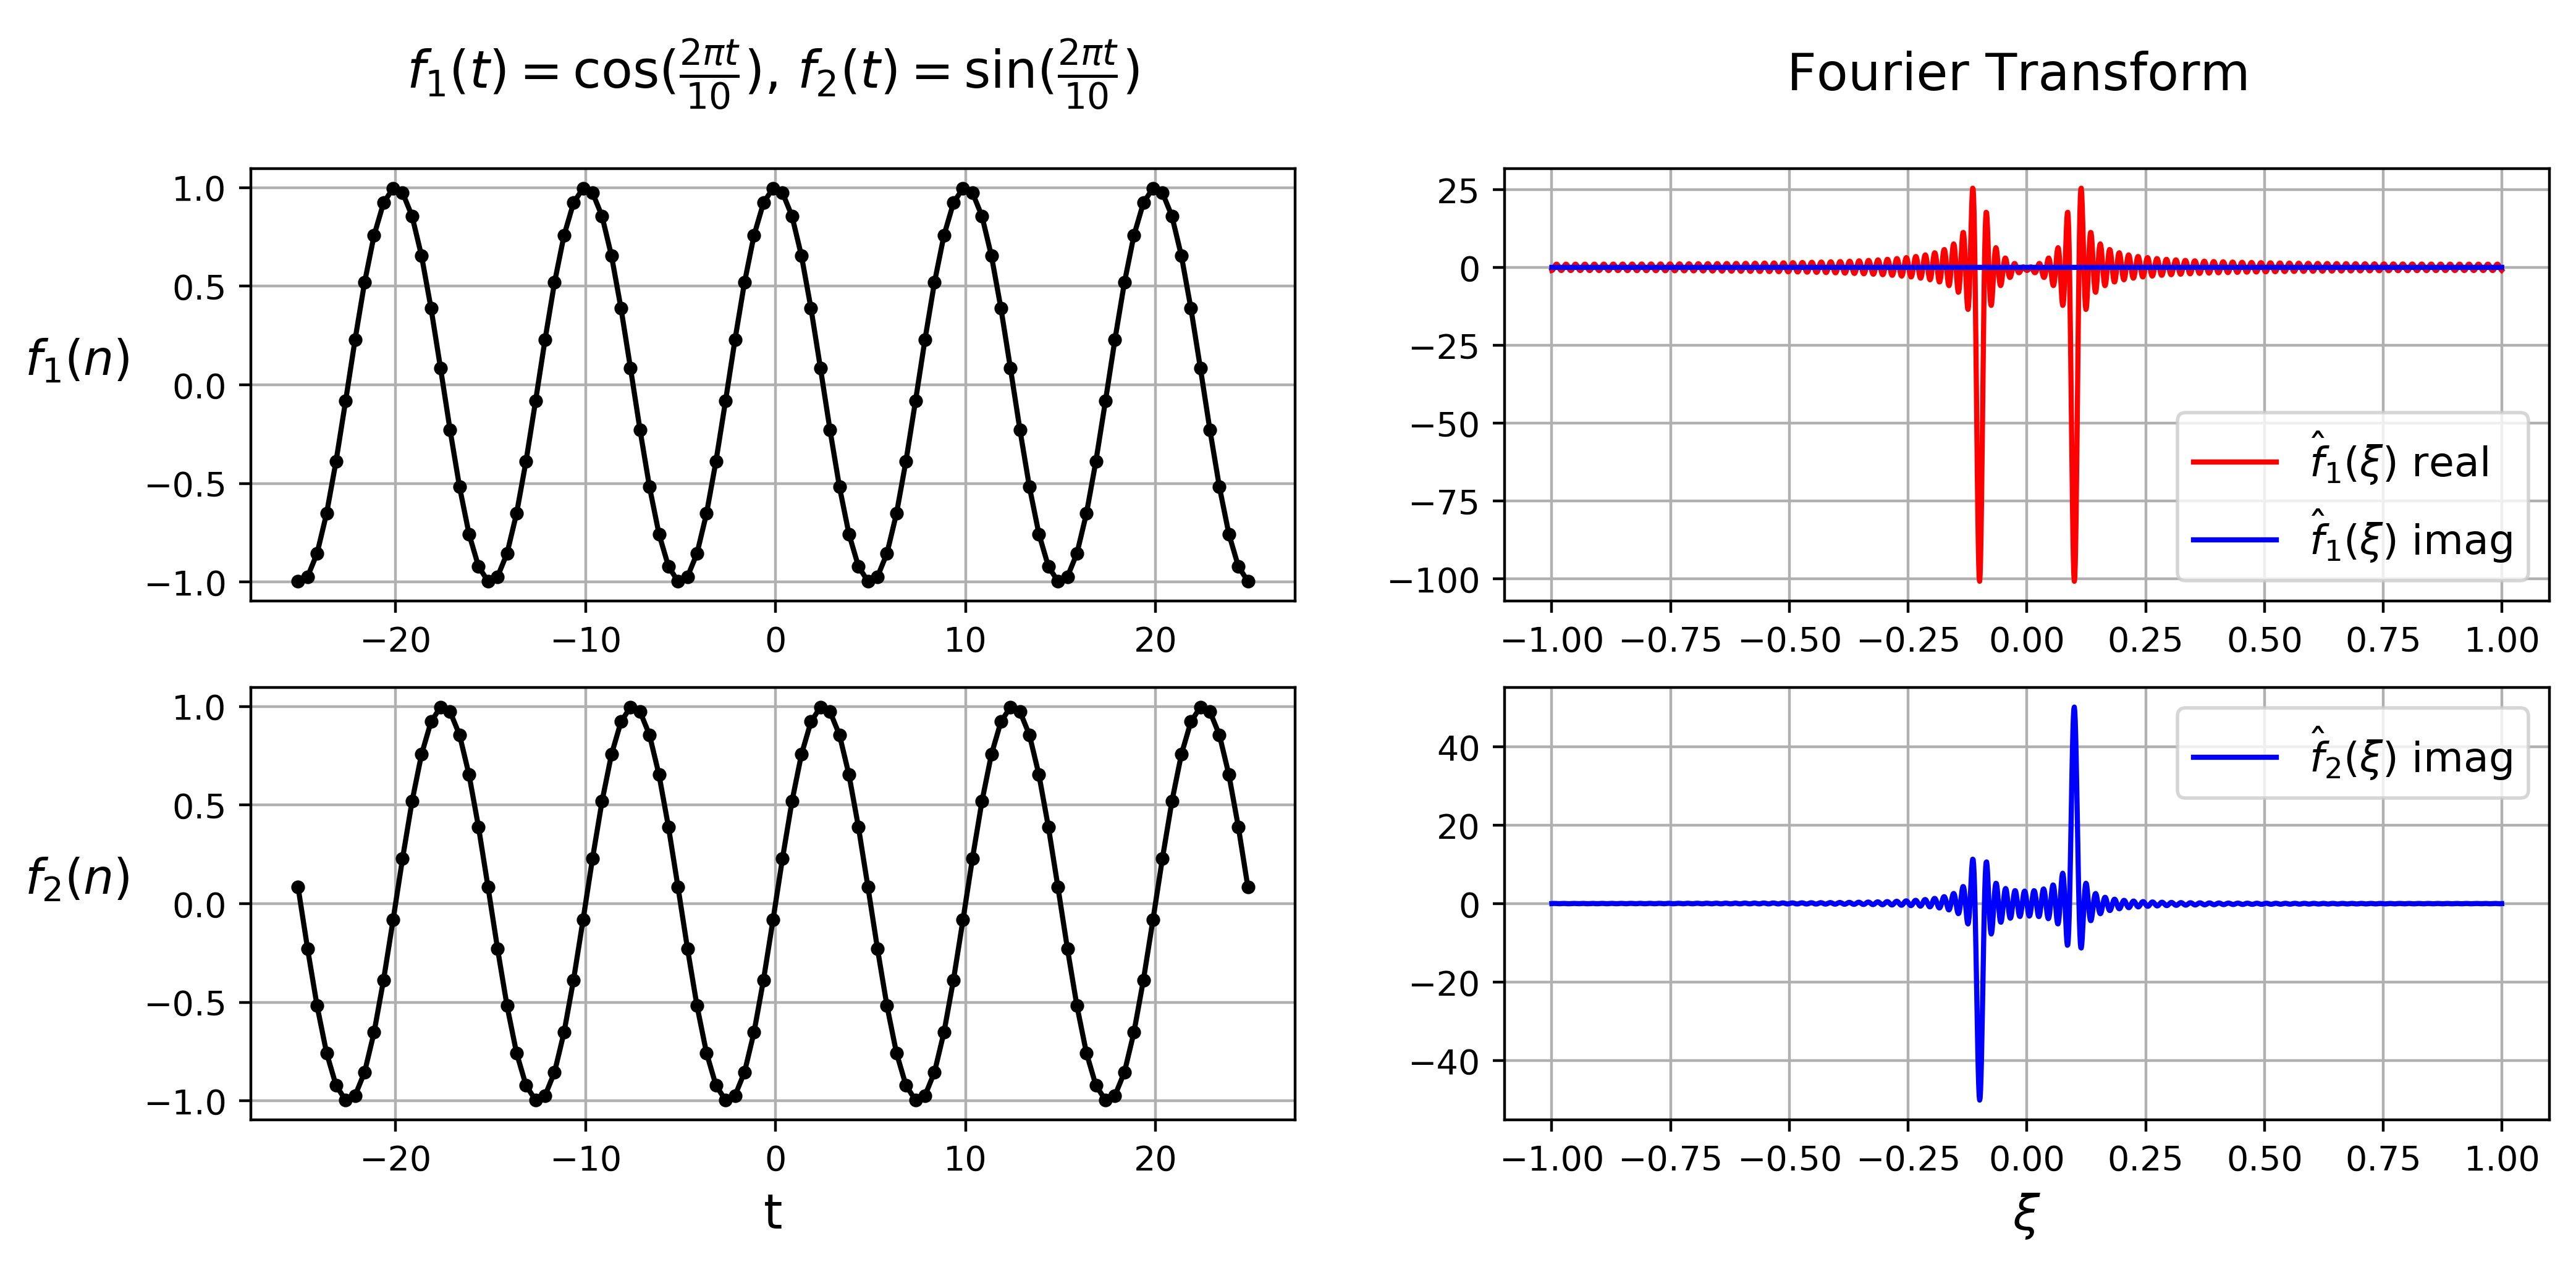
\includegraphics{../scripts/exercicio5/ft_symetries_real_trig.jpg}}	
	\end{center}
	\vspace{-2mm}	% acrescentar o espaçamento vertical apropriado entre a borda inferior da figura e a legenda ou a fonte quando não há legenda (o valor pode ser negativo para subir)
	%\legenda{Figura 1.1: Dez sinais e seus respectivos histogramas para  asérie com $N$ = 64 do grupo noise.}	% legenda - para deixar sem legenda usar comando \legenda{} (nunca deve-se comentar o comando \legenda)
	\label{ex1_fig1}
	%\FONTE{}	% fonte consultada (elemento obrigatório, mesmo que seja produção do próprio autor)
\end{figure}

\begin{figure}[ht!]
	\legenda{Figura 5.2: Transformada de Fourier de duas funções trigonométricas imaginárias, uma par e outra ímpar. A transformada da primeira é imaginária e par, já da segunda é real e ímpar.}
	\vspace{-1mm}	% acrescentar o espaçamento vertical apropriado entre o título e a borda superior da figura
	\begin{center}
		\resizebox{\textwidth}{!}{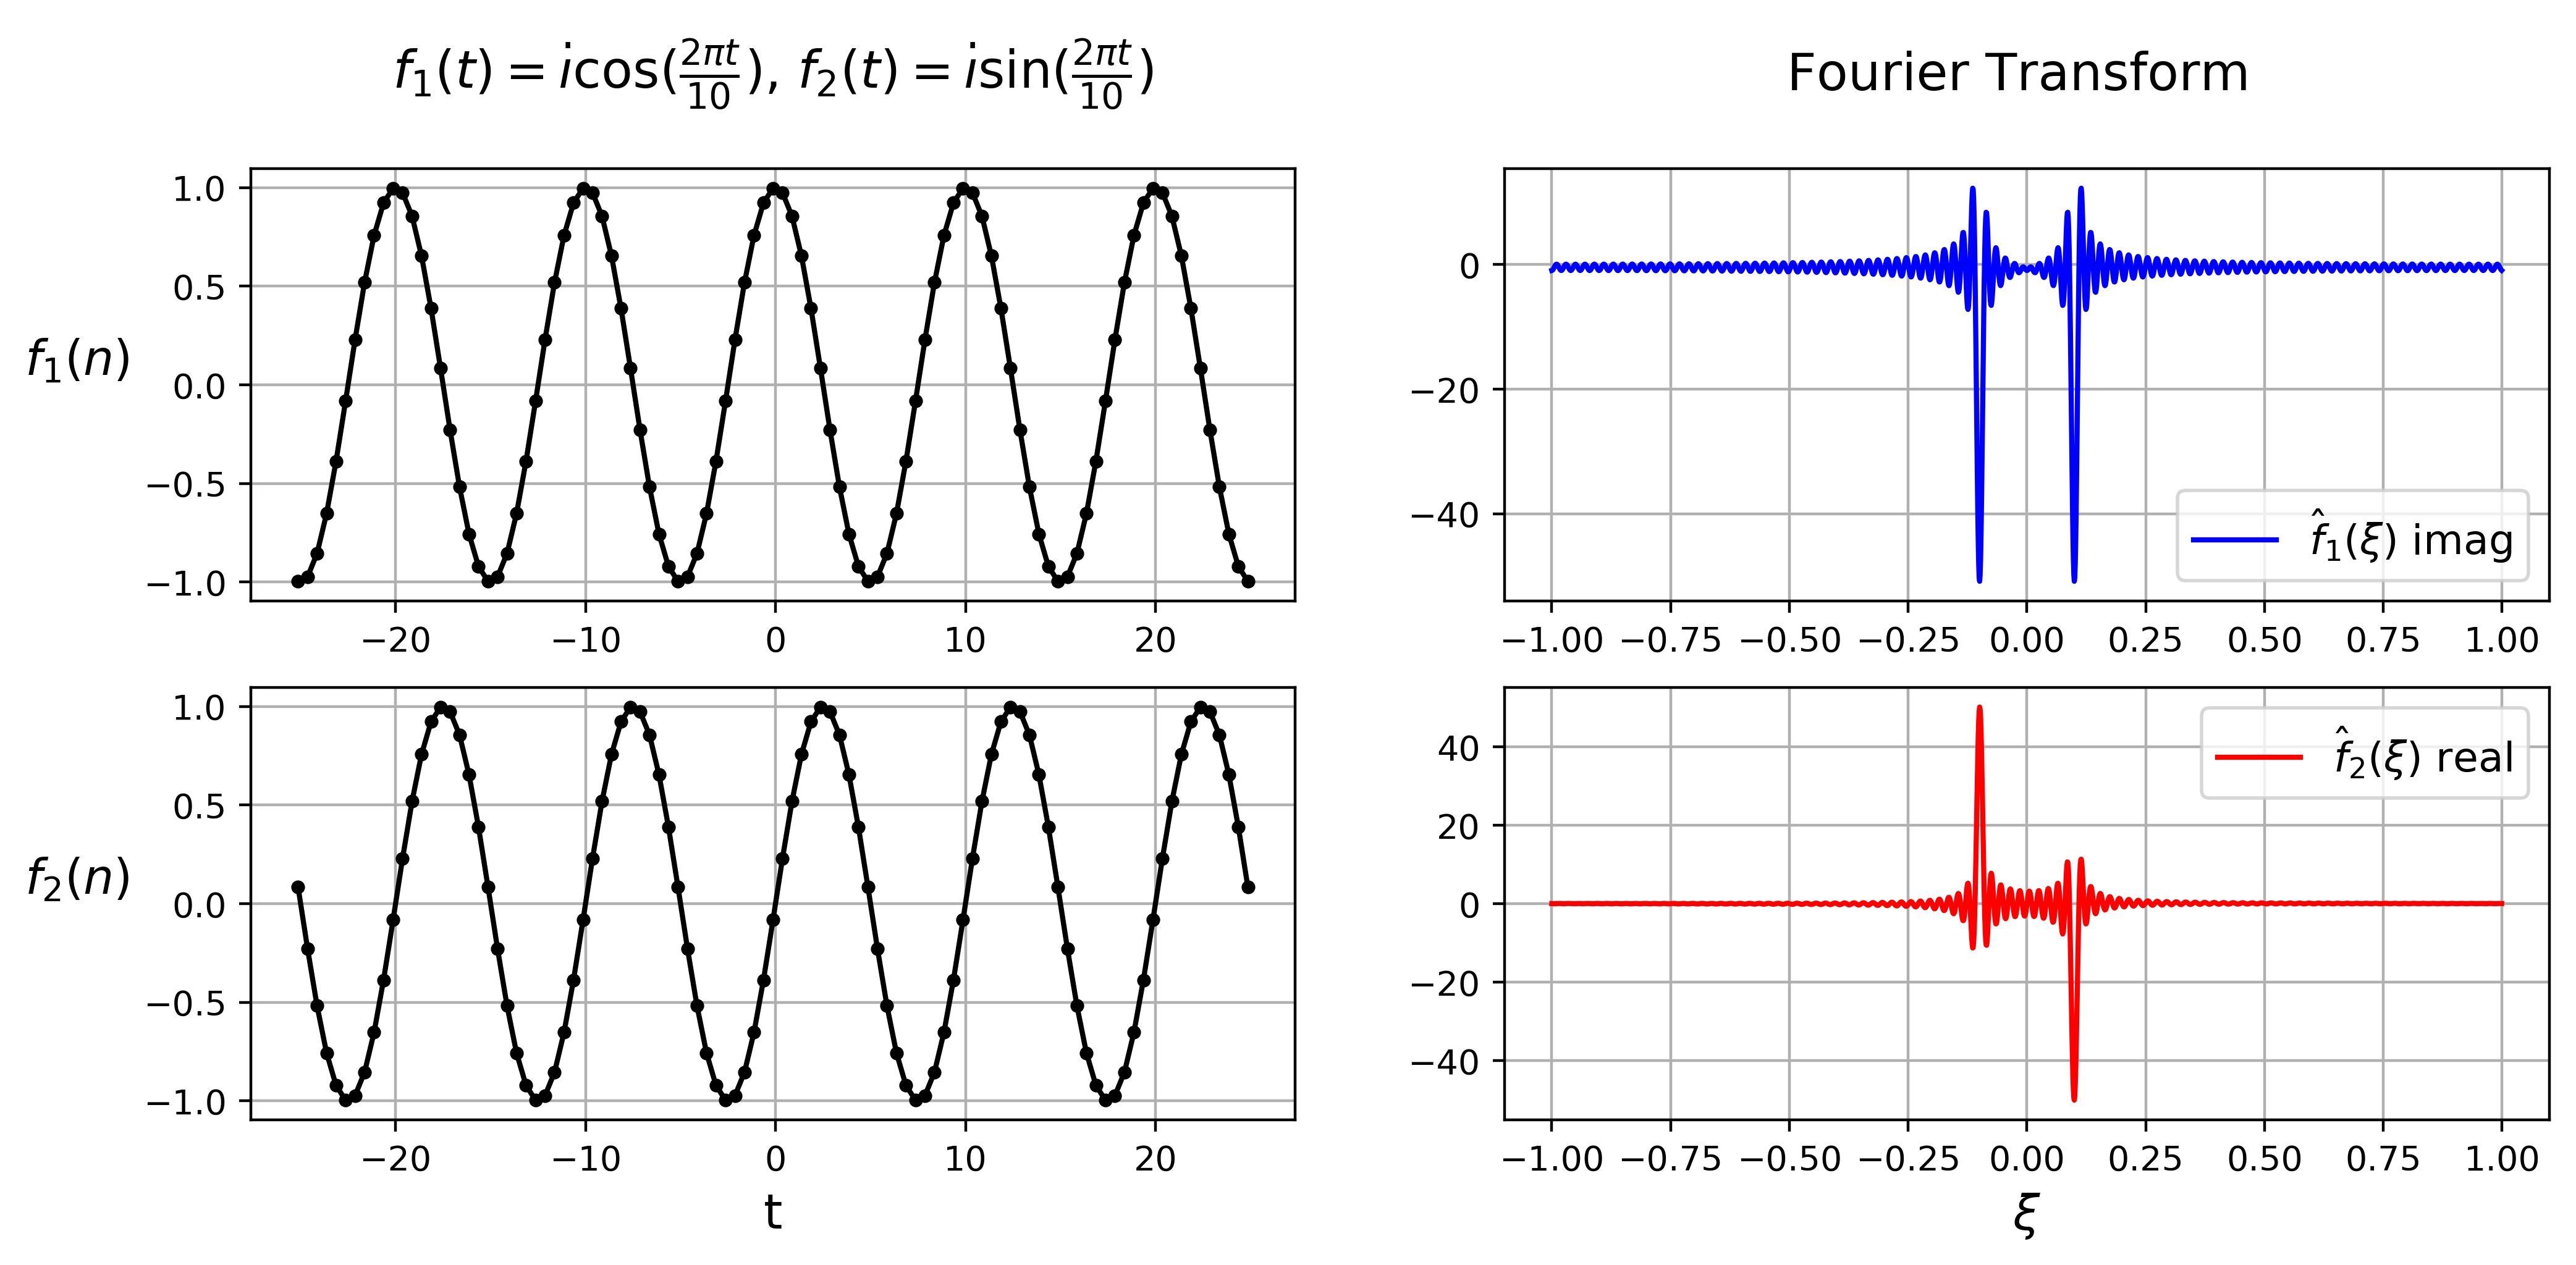
\includegraphics{../scripts/exercicio5/ft_symetries_imag_trig.jpg}}	
	\end{center}
	\vspace{-2mm}	% acrescentar o espaçamento vertical apropriado entre a borda inferior da figura e a legenda ou a fonte quando não há legenda (o valor pode ser negativo para subir)
	%\legenda{Figura 1.1: Dez sinais e seus respectivos histogramas para  asérie com $N$ = 64 do grupo noise.}	% legenda - para deixar sem legenda usar comando \legenda{} (nunca deve-se comentar o comando \legenda)
	\label{ex1_fig1}
	%\FONTE{}	% fonte consultada (elemento obrigatório, mesmo que seja produção do próprio autor)
\end{figure}

%============================ polys

\begin{figure}[ht!]
	\legenda{Figura 5.3: Transformada de Fourier de duas funções polinomiais reais, uma par e outra ímpar. A transformada da primeira é real e par, já da segunda é imaginária e ímpar.}
	\vspace{-1mm}	% acrescentar o espaçamento vertical apropriado entre o título e a borda superior da figura
	\begin{center}
		\resizebox{\textwidth}{!}{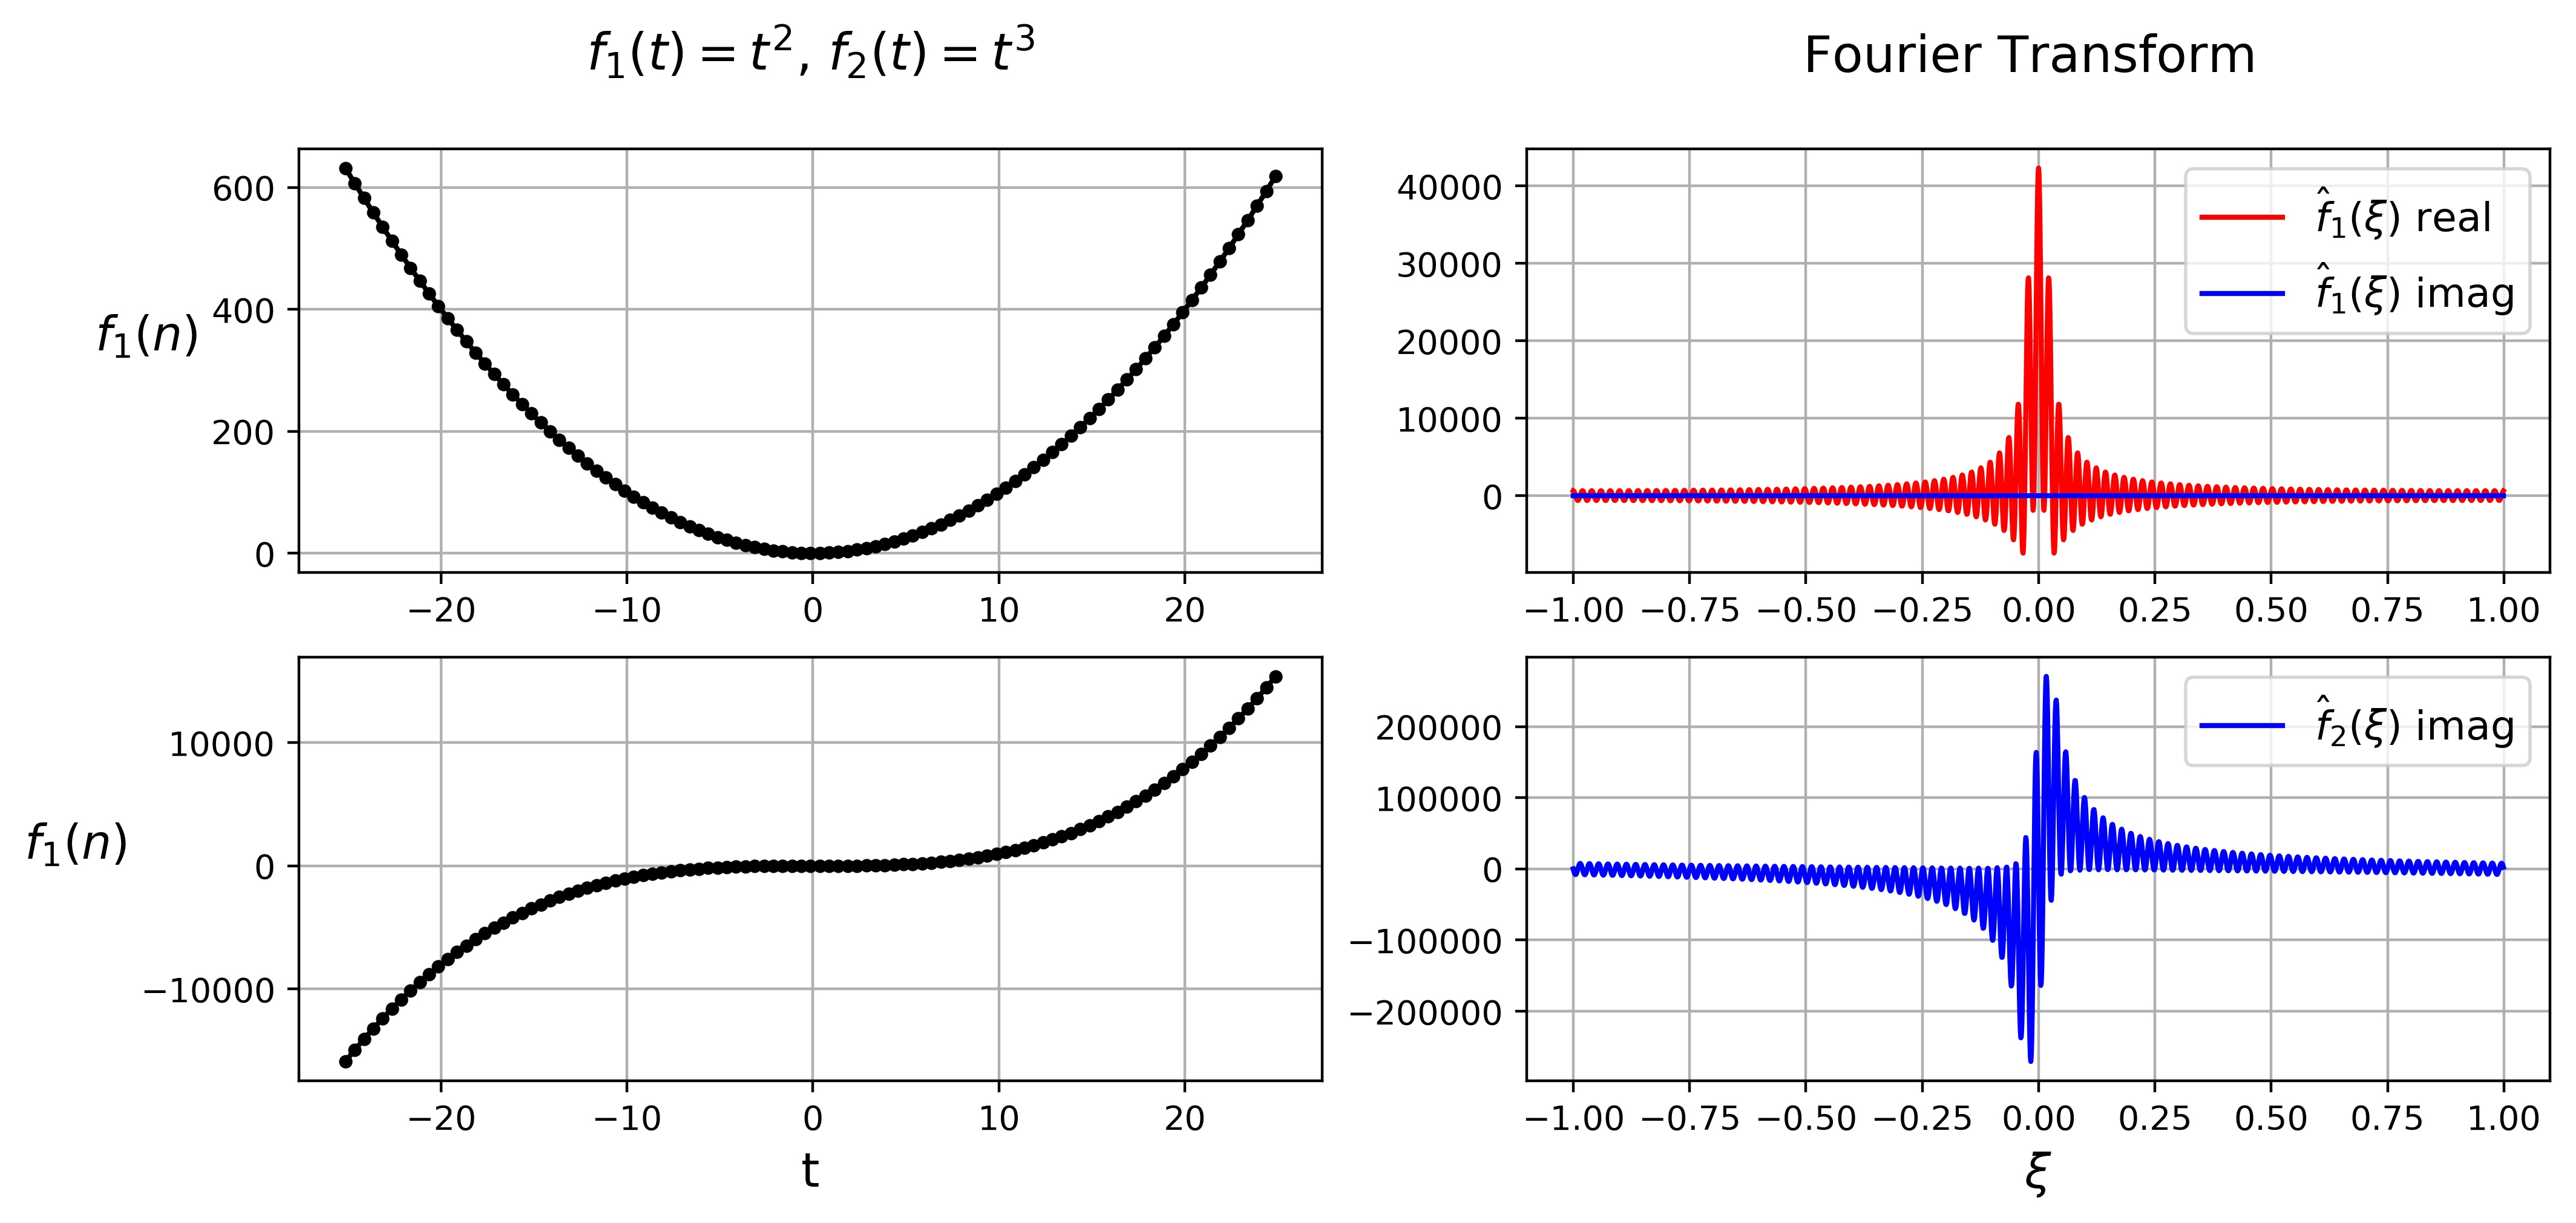
\includegraphics{../scripts/exercicio5/ft_symetries_real_poly.jpg}}	
	\end{center}
	\vspace{-2mm}	% acrescentar o espaçamento vertical apropriado entre a borda inferior da figura e a legenda ou a fonte quando não há legenda (o valor pode ser negativo para subir)
	%\legenda{Figura 1.1: Dez sinais e seus respectivos histogramas para  asérie com $N$ = 64 do grupo noise.}	% legenda - para deixar sem legenda usar comando \legenda{} (nunca deve-se comentar o comando \legenda)
	\label{ex1_fig1}
	%\FONTE{}	% fonte consultada (elemento obrigatório, mesmo que seja produção do próprio autor)
\end{figure}

\begin{figure}[ht!]
	\legenda{Figura 5.4: Transformada de Fourier de duas funções polinomiais imaginárias, uma par e outra ímpar. A transformada da primeira é imaginária e par, já da segunda é real e ímpar.}
	\vspace{-1mm}	% acrescentar o espaçamento vertical apropriado entre o título e a borda superior da figura
	\begin{center}
		\resizebox{\textwidth}{!}{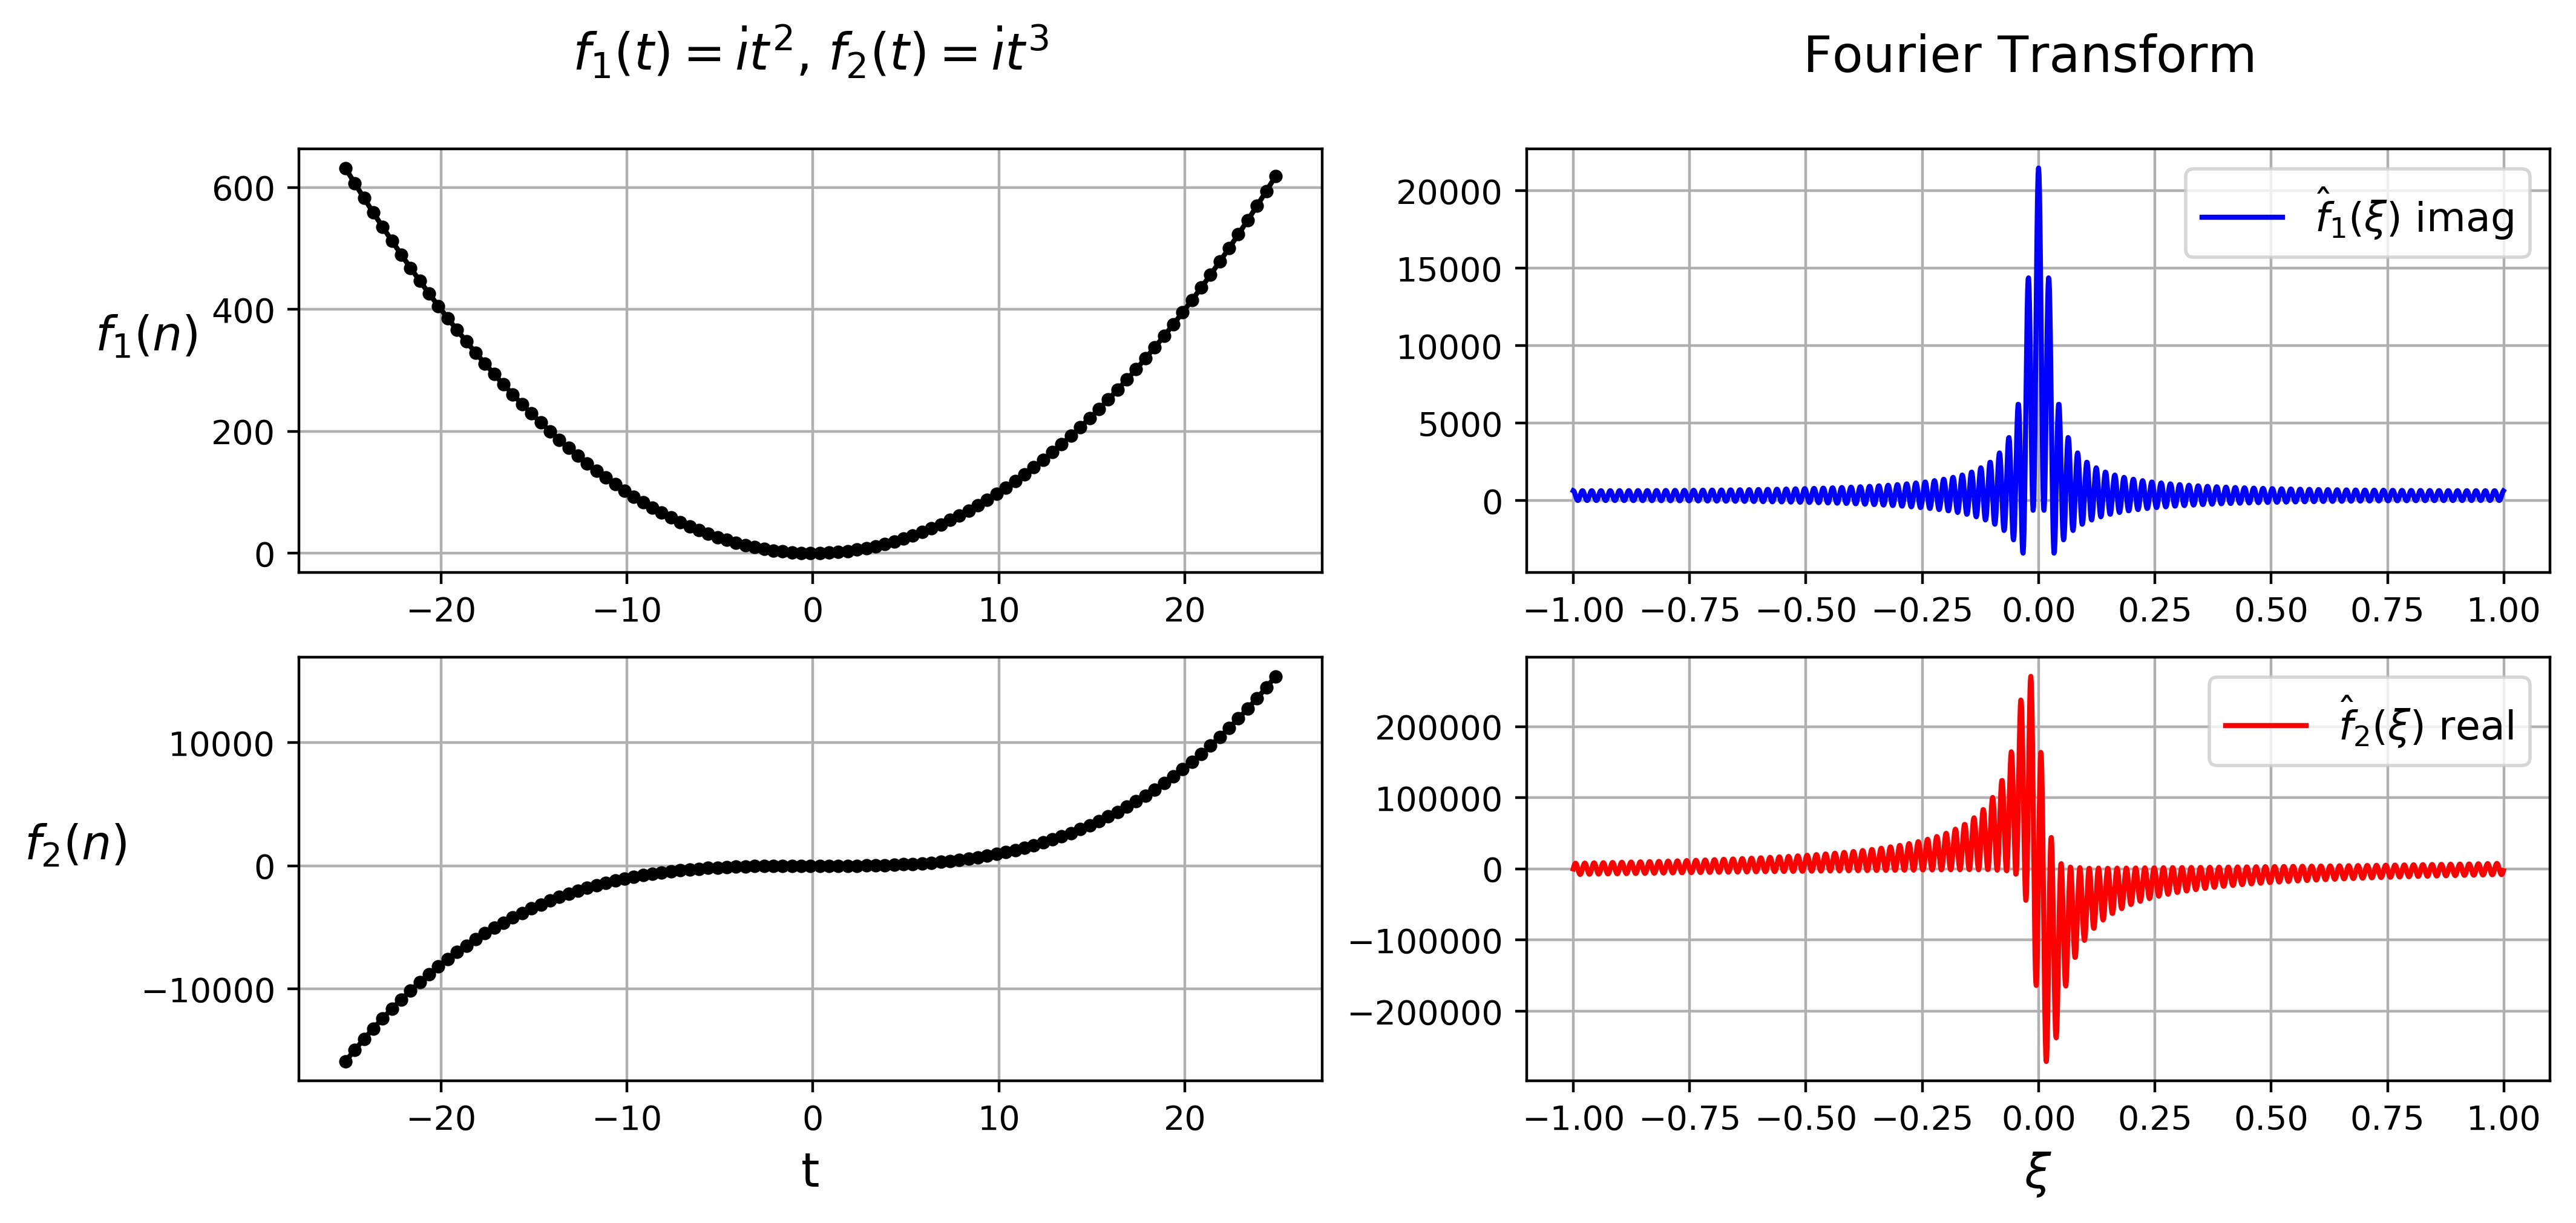
\includegraphics{../scripts/exercicio5/ft_symetries_imag_poly.jpg}}	
	\end{center}
	\vspace{-2mm}	% acrescentar o espaçamento vertical apropriado entre a borda inferior da figura e a legenda ou a fonte quando não há legenda (o valor pode ser negativo para subir)
	%\legenda{Figura 1.1: Dez sinais e seus respectivos histogramas para  asérie com $N$ = 64 do grupo noise.}	% legenda - para deixar sem legenda usar comando \legenda{} (nunca deve-se comentar o comando \legenda)
	\label{ex1_fig1}
	%\FONTE{}	% fonte consultada (elemento obrigatório, mesmo que seja produção do próprio autor)
\end{figure}
% EXEMPLO PARA ADICIONAR FIGURA
%\begin{figure}[ht!]
	%\caption{Série e histogramas.}
%	\vspace{0mm}	% acrescentar o espaçamento vertical apropriado entre o título e a borda superior da figura
%	\begin{center}
%		\resizebox{15cm}{!}{\includegraphics{Figuras/ex1/Exercicio1_n_64.jpg}}		
%	\end{center}
%	\vspace{-2mm}	% acrescentar o espaçamento vertical apropriado entre a borda inferior da figura e a legenda ou a fonte quando não há legenda (o valor pode ser negativo para subir)
%	\legenda{Figura 1.1: Dez sinais e seus respectivos histogramas para  asérie com $N$ = 64 do grupo noise.}	% legenda - para deixar sem legenda usar comando \legenda{} (nunca deve-se comentar o comando \legenda)
%	\label{ex1_fig1}
%	%\FONTE{}	% fonte consultada (elemento obrigatório, mesmo que seja produção do próprio autor)
%\end{figure}
